
% Decomposition example of n=5 = 2+1+2



\begin{center}
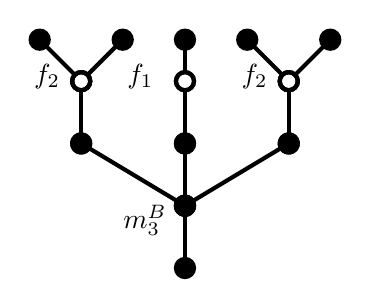
\begin{tikzpicture}[x=0.75pt,y=0.75pt,yscale=-1,xscale=1]
%uncomment if require: \path (0,513); %set diagram left start at 0, and has height of 513

%Straight Lines [id:da7617349086666938] 
\draw [line width=1.5]    (130,120) -- (80,90) ;
\draw [shift={(80,90)}, rotate = 210.96] [color={rgb, 255:red, 0; green, 0; blue, 0 }  ][fill={rgb, 255:red, 0; green, 0; blue, 0 }  ][line width=1.5]      (0, 0) circle [x radius= 4.36, y radius= 4.36]   ;
\draw [shift={(130,120)}, rotate = 210.96] [color={rgb, 255:red, 0; green, 0; blue, 0 }  ][fill={rgb, 255:red, 0; green, 0; blue, 0 }  ][line width=1.5]      (0, 0) circle [x radius= 4.36, y radius= 4.36]   ;
%Straight Lines [id:da44963436792962175] 
\draw [line width=1.5]    (130,120) -- (180,90) ;
\draw [shift={(180,90)}, rotate = 329.04] [color={rgb, 255:red, 0; green, 0; blue, 0 }  ][fill={rgb, 255:red, 0; green, 0; blue, 0 }  ][line width=1.5]      (0, 0) circle [x radius= 4.36, y radius= 4.36]   ;
\draw [shift={(130,120)}, rotate = 329.04] [color={rgb, 255:red, 0; green, 0; blue, 0 }  ][fill={rgb, 255:red, 0; green, 0; blue, 0 }  ][line width=1.5]      (0, 0) circle [x radius= 4.36, y radius= 4.36]   ;
%Straight Lines [id:da38320038561323777] 
\draw [line width=1.5]    (130,150) -- (130,120) ;
\draw [shift={(130,120)}, rotate = 270] [color={rgb, 255:red, 0; green, 0; blue, 0 }  ][fill={rgb, 255:red, 0; green, 0; blue, 0 }  ][line width=1.5]      (0, 0) circle [x radius= 4.36, y radius= 4.36]   ;
\draw [shift={(130,150)}, rotate = 270] [color={rgb, 255:red, 0; green, 0; blue, 0 }  ][fill={rgb, 255:red, 0; green, 0; blue, 0 }  ][line width=1.5]      (0, 0) circle [x radius= 4.36, y radius= 4.36]   ;
%Straight Lines [id:da808520182955266] 
\draw [line width=1.5]    (77.63,57.63) -- (60,40) ;
\draw [shift={(60,40)}, rotate = 225] [color={rgb, 255:red, 0; green, 0; blue, 0 }  ][fill={rgb, 255:red, 0; green, 0; blue, 0 }  ][line width=1.5]      (0, 0) circle [x radius= 4.36, y radius= 4.36]   ;
\draw [shift={(80,60)}, rotate = 225] [color={rgb, 255:red, 0; green, 0; blue, 0 }  ][line width=1.5]      (0, 0) circle [x radius= 4.36, y radius= 4.36]   ;
%Straight Lines [id:da3918543796508074] 
\draw [line width=1.5]    (82.37,57.63) -- (100,40) ;
\draw [shift={(100,40)}, rotate = 315] [color={rgb, 255:red, 0; green, 0; blue, 0 }  ][fill={rgb, 255:red, 0; green, 0; blue, 0 }  ][line width=1.5]      (0, 0) circle [x radius= 4.36, y radius= 4.36]   ;
\draw [shift={(80,60)}, rotate = 315] [color={rgb, 255:red, 0; green, 0; blue, 0 }  ][line width=1.5]      (0, 0) circle [x radius= 4.36, y radius= 4.36]   ;
%Straight Lines [id:da6167040128706918] 
\draw [line width=1.5]    (80,86.65) -- (80,63.36) ;
\draw [shift={(80,60)}, rotate = 270] [color={rgb, 255:red, 0; green, 0; blue, 0 }  ][line width=1.5]      (0, 0) circle [x radius= 4.36, y radius= 4.36]   ;
\draw [shift={(80,90)}, rotate = 270] [color={rgb, 255:red, 0; green, 0; blue, 0 }  ][line width=1.5]      (0, 0) circle [x radius= 4.36, y radius= 4.36]   ;
%Straight Lines [id:da030465125332191922] 
\draw [line width=1.5]    (130,86.65) -- (130,63.36) ;
\draw [shift={(130,60)}, rotate = 270] [color={rgb, 255:red, 0; green, 0; blue, 0 }  ][line width=1.5]      (0, 0) circle [x radius= 4.36, y radius= 4.36]   ;
\draw [shift={(130,90)}, rotate = 270] [color={rgb, 255:red, 0; green, 0; blue, 0 }  ][line width=1.5]      (0, 0) circle [x radius= 4.36, y radius= 4.36]   ;
%Straight Lines [id:da3974786996509143] 
\draw [line width=1.5]    (130,56.65) -- (130,40) ;
\draw [shift={(130,40)}, rotate = 270] [color={rgb, 255:red, 0; green, 0; blue, 0 }  ][fill={rgb, 255:red, 0; green, 0; blue, 0 }  ][line width=1.5]      (0, 0) circle [x radius= 4.36, y radius= 4.36]   ;
\draw [shift={(130,60)}, rotate = 270] [color={rgb, 255:red, 0; green, 0; blue, 0 }  ][line width=1.5]      (0, 0) circle [x radius= 4.36, y radius= 4.36]   ;
%Straight Lines [id:da37381963954525443] 
\draw [line width=1.5]    (130,120) -- (130,90) ;
\draw [shift={(130,90)}, rotate = 270] [color={rgb, 255:red, 0; green, 0; blue, 0 }  ][fill={rgb, 255:red, 0; green, 0; blue, 0 }  ][line width=1.5]      (0, 0) circle [x radius= 4.36, y radius= 4.36]   ;
\draw [shift={(130,120)}, rotate = 270] [color={rgb, 255:red, 0; green, 0; blue, 0 }  ][fill={rgb, 255:red, 0; green, 0; blue, 0 }  ][line width=1.5]      (0, 0) circle [x radius= 4.36, y radius= 4.36]   ;
%Straight Lines [id:da26767039393186676] 
\draw [line width=1.5]    (177.63,57.63) -- (160,40) ;
\draw [shift={(160,40)}, rotate = 225] [color={rgb, 255:red, 0; green, 0; blue, 0 }  ][fill={rgb, 255:red, 0; green, 0; blue, 0 }  ][line width=1.5]      (0, 0) circle [x radius= 4.36, y radius= 4.36]   ;
\draw [shift={(180,60)}, rotate = 225] [color={rgb, 255:red, 0; green, 0; blue, 0 }  ][line width=1.5]      (0, 0) circle [x radius= 4.36, y radius= 4.36]   ;
%Straight Lines [id:da6867187917151945] 
\draw [line width=1.5]    (182.37,57.63) -- (200,40) ;
\draw [shift={(200,40)}, rotate = 315] [color={rgb, 255:red, 0; green, 0; blue, 0 }  ][fill={rgb, 255:red, 0; green, 0; blue, 0 }  ][line width=1.5]      (0, 0) circle [x radius= 4.36, y radius= 4.36]   ;
\draw [shift={(180,60)}, rotate = 315] [color={rgb, 255:red, 0; green, 0; blue, 0 }  ][line width=1.5]      (0, 0) circle [x radius= 4.36, y radius= 4.36]   ;
%Straight Lines [id:da9667052161881513] 
\draw [line width=1.5]    (180,86.65) -- (180,63.36) ;
\draw [shift={(180,60)}, rotate = 270] [color={rgb, 255:red, 0; green, 0; blue, 0 }  ][line width=1.5]      (0, 0) circle [x radius= 4.36, y radius= 4.36]   ;
\draw [shift={(180,90)}, rotate = 270] [color={rgb, 255:red, 0; green, 0; blue, 0 }  ][line width=1.5]      (0, 0) circle [x radius= 4.36, y radius= 4.36]   ;

% Text Node
\draw (101,50.4) node [anchor=north west][inner sep=0.75pt]    {$f_{1}$};
% Text Node
\draw (56,50.4) node [anchor=north west][inner sep=0.75pt]    {$f_{2}$};
% Text Node
\draw (99,118.4) node [anchor=north west][inner sep=0.75pt]    {$m^{B}_{3}$};
% Text Node
\draw (156,50.4) node [anchor=north west][inner sep=0.75pt]    {$f_{2}$};


\end{tikzpicture}    
\end{center}